\chapter{Background}
The methods developed in this thesis build on foundational concepts from \gls{rl}, \gls{marl}, and quadrotor dynamics. We first review model-free, on-policy policy-optimization algorithms, introducing \gls{mdp}s, policy gradients, and \gls{ppo}. We then extend these ideas to cooperative multi-agent tasks, comparing centralized critics with fully decentralized critics. Next, we present the mathematical model of a quadrotor \gls{uav}, covering coordinate frames, state representation, sensor fusion, continuous-time dynamics, and common action-space formulations ranging from velocity commands to direct thrust control. Finally, we explain how the quadrotor state is augmented to include cable-suspended payloads—first via a simple pendulum model and then through multi-link or tendon-based approximations—and how these formulations generalize to cooperative transport by multiple \glspl{uav}. These elements are essential for developing a deep \gls{rl} framework for decentralized multi-\gls{uav} cable-suspended payload transport.

\section{\glsxtrfull{rl}}
\glsxtrfull{rl} refers to algorithms that learn to make decisions by interacting with an environment through trial-and-error exploration, gradually improving behavior based on received feedback. These methods have been successfully applied to a wide range of sequential decision-making problems, including robotics control, game playing, and resource management \cite{mnih2015human}. \gls{rl} algorithms can be broadly categorized into model-free and model-based approaches, as well as on-policy and off-policy methods, each offering different trade-offs between sample efficiency and stability \cite{Schulman2015TrustRP}.  

Model-free methods learn policies or value functions directly from observed interactions without constructing an explicit model of the environment's dynamics. This simplifies implementation and avoids model bias, but often requires more data to converge compared to model-based approaches.  

This work focuses on model-free, on-policy, policy-optimization methods, where the policy used to collect data is the same one being updated. For a comprehensive treatment of \gls{rl} fundamentals, see \cite{SuttonBarto2018}.
\subsection{Fundamentals}
Before introducing the specific algorithm, we first define the key concepts and ideas of \gls{rl}.
\paragraph{Markov Decision Processes}

\begin{figure}
\centering
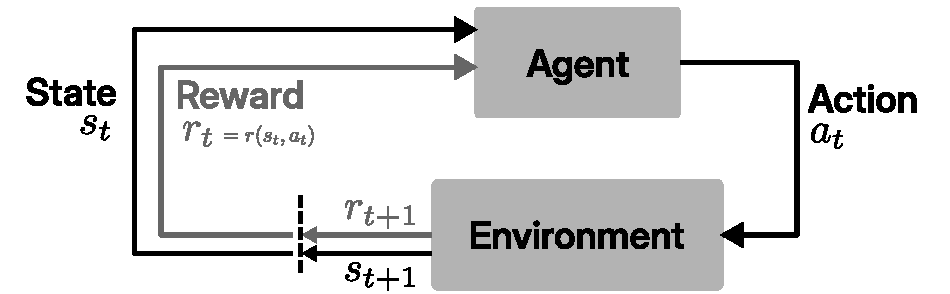
\includegraphics[width=0.8\textwidth]{images/figs/rl.pdf}
\caption[\gls{rl} framework]{\gls{rl} framework. The agent interacts with the environment by taking actions and receiving rewards, while the environment transitions to new states based on the agent's actions.}
\label{fig:rl_diagram}
\end{figure}

\gls{rl} problems are commonly framed as \gls{mdp}s, defined by the tuple \((\mathcal{S}, \mathcal{A}, P, r, \rho_0, \gamma)\), where \(\mathcal{S}\) is the set of states, \(\mathcal{A}\) is the set of actions, \(P(s_{t+1}\!\mid\!s_t,a_t)\) is the transition probability, \(r(s_t,a_t)\) is the immediate reward, \(\gamma \in [0,1)\) is the discount factor, and \(\rho_0\) is the initial state distribution with \(s_0 \sim \rho_0\). At each time step \(t\), the agent observes \(s_t\), samples and executes \(a_t \sim \pi_\theta(\cdot\mid s_t)\), receives \(r_t = r(s_t,a_t)\), and transitions to \(s_{t+1} \sim P(\cdot\mid s_t,a_t)\). This procedure is visualized in figure \ref{fig:rl_diagram}. In practice, the agent often has access only to a partial observation \(o_t\). We use \(o_t\) or \(s_t\) interchangeably depending on context.

\paragraph{Policies}
The agent's behavior is defined by a policy \(\pi_{\theta}\), parameterized by \(\theta \in \mathbb{R}^{d}\). A deterministic policy outputs
$ 
a_t = \pi_{\theta}(s_t),
$
while a stochastic policy samples
$
a_t \sim \pi_{\theta}(\,\cdot\mid s_t).
$
We optimize \(\pi_\theta\) to maximize the expected return, typically representing it as a neural network mapping states to action distributions.

\paragraph{Reward and Return}
The agent's goal is to maximize the expected return, which is the total discounted reward over time. 
The reward function \(r_t=r(s_t,a_t)\) provides immediate feedback to the agent and usually depends on the current state \(s_t\), action taken by the policy \(a_t\) and the next state \(s_{t+1}\). The discounted return from the start is defined as
\begin{equation}
R_0 = \sum_{t=0}^{\infty} \gamma^t r_t\,,
\end{equation}
where \(\gamma\) is the discount factor that determines the importance of future rewards. The expected return \(J(\pi)\) is defined as the expected value of the discounted return
\begin{equation}
J(\pi) = \mathbb{E}\bigl[R_0\bigr]
= \mathbb{E}\Bigl[\sum_{t=0}^\infty \gamma^t r_t\Bigr].
\end{equation}
and the goal is to find \(\pi^* = \arg\max_\pi J(\pi)\). Formally,
\begin{equation}\label{eq:RL_opt}
\begin{aligned}
\text{maximize} \quad & \mathbb{E}\Bigl[\sum_{t=0}^\infty \gamma^t\,r(s_t,a_t)\Bigr] \\
\text{subject to} \quad & s_0 \sim \rho_0, \quad a_t \sim \pi(\cdot\mid s_t), \quad s_{t+1} \sim P(\cdot\mid s_t,a_t).
\end{aligned}
\end{equation}

\paragraph{Value and Action-Value Functions}
Under a fixed policy \(\pi_\theta\), the state-value function \(V^\pi(s_t)\) and the action-value function \(Q^\pi(s_t,a_t)\) measure the expected discounted return:
\begin{equation}
V^\pi(s_t) = \mathbb{E}\Bigl[\sum_{t=0}^\infty \gamma^t r_t \;\big|\; s_0 = s_t\Bigr], 
\qquad
Q^\pi(s_t,a_t) = \mathbb{E}\Bigl[\sum_{t=0}^\infty \gamma^t r_t \;\big|\; s_0 = s_t,\,a_0 = a_t\Bigr].
\end{equation}

Here, \(V^\pi(s_t)\) is the expected discounted return starting from state \(s_t\) under \(\pi_\theta\), and \(Q^\pi(s_t,a_t)\) is the expected discounted return starting from \(s_t\), taking action \(a_t\), then following \(\pi_\theta\).
The Bellman equations decompose these functions into immediate reward plus the discounted value of the subsequent state:
\begin{align}
V^\pi(s_t)
&= \mathbb{E}_{a_t\sim\pi(\cdot\mid s_t)}\bigl[r(s_t,a_t)\bigr]
  + \gamma\,\mathbb{E}_{s_{t+1}\sim P(\cdot\mid s_t,a_t)}\bigl[V^\pi(s_{t+1})\bigr],\\
Q^\pi(s_t,a_t)
&= \mathbb{E}_{s_{t+1}\sim P(\cdot\mid s_t,a_t)}\bigl[r(s_t,a_t)\bigr]
  + \gamma\,\mathbb{E}_{a_{t+1}\sim\pi(\cdot\mid s_{t+1})}\bigl[Q^\pi(s_{t+1},a_{t+1})\bigr].
\end{align}
The advantage function \(A^\pi(s_t,a_t)\) quantifies the relative value of taking action \(a_t\) in state \(s_t\) compared to the average value of \(s_t\):
\begin{equation}
A^\pi(s_t,a_t) = Q^\pi(s_t,a_t) - V^\pi(s_t).
\end{equation}

\paragraph{On-Policy Policy-Gradient Methods}
On-policy methods collect data under the current policy \(\pi_\theta\) and perform gradient ascent on \(J(\theta)\) to ultimately improve the policy towards \(\pi^*\). The policy gradient can be expressed using the advantage function:
\begin{equation}
\nabla_\theta J(\theta)
= \mathbb{E}\Bigl[\sum_{t=0}^\infty \gamma^t \,\nabla_\theta \log \pi_\theta(a_t\mid s_t)\,\hat A_t\Bigr].
\end{equation}
In practice, there are different approaches to approximate the policy gradient \(\nabla_{\theta}J(\theta)\). In the next section, we will focus on the \gls{ppo} algorithm, which is a popular on-policy method, using a surrogate objective function to optimize the policy.
\subsection{Proximal Policy Optimization}
\gls{ppo} \cite{schulman2017proximal} alternates between sampling trajectories using the current policy and performing multiple epochs of stochastic gradient ascent on a clipped surrogate objective. For continuous control, the actor network outputs parameters of a Gaussian distribution,
\begin{equation}
a_t \sim \mathcal{N}\bigl(\mu_\theta(s_t),\,\sigma_\theta(s_t)\bigr),
\end{equation}
Here, the actor network (parameterized by \(\theta\)) maps a state \(s_t\) to a distribution over actions, thereby defining the policy \(\pi_\theta(a_t \mid s_t)\). This stochastic sampling is crucial as it enables the agent to explore a continuous range of actions, promoting both exploration and robustness in learning.

\gls{ppo} builds on the actor-critic framework, where two neural networks, the actor network and the critic network, are optimized simultaneously. The actor network, or policy network, directly outputs the action probabilities or probability distribution. The critic network, often parameterized by \(\phi\), estimates a value function \(V_\phi(s_t)\) that evaluates the quality of states, or more precisely the expected return from \(s_t\) under the current policy. The critic's estimate is used to compute an advantage function that quantifies the relative benefit of taking a specific action in a given state. A commonly used method for estimating advantages is \gls{gae}, which effectively reduces variance while introducing a manageable bias that aids learning stability. \gls{gae} computes the advantage as
\begin{equation}
\hat{A}_t = \sum_{l=0}^{\infty} (\gamma \lambda)^l \delta_{t+l}, 
\quad
\delta_t = r_t + \gamma V_\phi(s_{t+1}) - V_\phi(s_t).
\end{equation}
Here, \(r_t\) is the reward received at time \(t\), \(V_\phi(s_t)\) is the estimated value of state \(s_t\) from the critic network under the current policy, \(\gamma \in [0,1]\) is the discount factor that weighs future rewards, and \(\lambda \in [0,1]\) is a parameter that adjusts the trade-off between bias and variance in the advantage estimates.

A key contribution of \gls{ppo} is the use of a clipped surrogate objective designed to restrict the size of policy updates. We can define the probability ratio between the new and the old policies
\begin{equation}
\rho_t(\theta) = \frac{\pi_\theta(a_t\mid s_t)}{\pi_{\theta_{\text{old}}}(a_t\mid s_t)},
\end{equation}
Now, the clipped surrogate objective is
\begin{equation}
L^{\text{CLIP}}(\theta) = \mathbb{E}_t\!\Bigl[\min\!\bigl(\rho_t(\theta)\,\hat{A}_t;\text{clip}(\rho_t(\theta),1-\epsilon,1+\epsilon)\,\hat{A}_t\bigr)\Bigr],
\end{equation}
where \(\hat{A}_t\) is an estimator of the advantage function and \(\epsilon\) is a hyperparameter defining the clipping range. This objective penalizes overly large deviations from the previous policy, ensuring that updates remain conservative while still allowing for meaningful improvements.

In practice, \gls{ppo} combines the policy surrogate loss with additional terms, such as a value function loss, which is computed by the critic network, and an entropy bonus, yielding a composite objective:
\begin{equation}
L(\theta,\phi) = \mathbb{E}_t\Bigl[L^{\text{CLIP}}(\theta)
  - c_1\,\bigl(V_\phi(s_t) - V_t^{\text{target}}\bigr)^2
  + c_2\,S\bigl[\pi_\theta(\cdot\mid s_t)\bigr]\Bigr],
\end{equation}
where \(c_1\) and \(c_2\) are coefficients that weight the contributions of the value function error and the entropy bonus \(S\big[\pi_\theta\big](s_t)\), respectively. The term \(\left(V_\phi(s_t) - V_t^{\text{target}}\right)^2\) is the critic's squared error against the target value \(V_t^{\text{target}}\). This final objective is optimized using stochastic gradient ascent over multiple epochs on the same batch of on-policy samples, updating both actor parameters \(\theta\) and critic parameters \(\phi\).

The overall procedure of \gls{ppo} in an actor-critic setting is summarized in Algorithm~\ref{alg:ppo}. In the algorithm, \(\theta\) denotes the current policy parameters, \(\theta_{\text{old}}\) are the parameters used for generating the on-policy data, \(U\) is the number of parallel actors (often parallel simulation environments), \(T\) is the number of timesteps per actor rollout (with \(UT\) total timesteps per batch), \(K\) is the number of epochs over the data, and \(M \le UT\) is the minibatch size. The critic network's parameters \(\phi\) are updated alongside \(\theta\) whenever the value loss term is backpropagated.

\begin{algorithm}[H]
\caption{Proximal Policy Optimization (Actor-Critic)}
\label{alg:ppo}
\begin{algorithmic}[1]
\For{iteration = 1, 2, \dots}
    \For{actor = 1, 2, \dots, U}
        \State Run policy \(\pi_{\theta_{\text{old}}}\) (actor network) in the environment for \(T\) timesteps.
        \State Compute advantage estimates \(\hat{A}_1, \dots, \hat{A}_T\) using the critic network's value estimates.
    \EndFor
    \State Optimize the composite loss \(L(\theta)\) with respect to \(\theta\) (for the actor) and update \(\phi\) (for the critic) using \(K\) epochs and minibatch size \(M \le UT\).
    \State Update \(\theta_{\text{old}} \leftarrow \theta\).
\EndFor
\end{algorithmic}
\end{algorithm}

Overall, \gls{ppo} strikes a favorable balance between simplicity and performance, making it one of the most widely adopted on-policy algorithms in modern \gls{rl} applications. The following sections will discuss the multi-agent extensions of \gls{ppo} that are used in this work.
\section{\glsxtrfull{marl}}
This section provides an overview of the theoretical background of \gls{marl} as applied in this work. Our work evaluates both centralized and decentralized training paradigms. In particular, we employ \gls{ppo} for centralized training, while also exploring decentralized approaches using \gls{ippo} and \gls{mappo}, which are detailed in subsequent sections.
\subsection{Multi-Agent Markov Decision Process}
A cooperative multi-agent \gls{rl} problem can be formalized as a \gls{dec-pomdp}\cite{oliehoek_concise_2016}, defined by the tuple
\begin{equation}
  \bigl(\mathcal{N},\,\mathcal{S},\,\{\mathcal{A}^i\}_{i=1}^N,\,P,\,r,\,\{\Omega^i\}_{i=1}^N,\,O,\,\rho_0,\,\gamma\bigr)
\end{equation}
where $\mathcal{N}=\{1,\dots,N\}$ is the set of agents; $\mathcal{S}$ is the set of global states (with $s_0\sim\rho(s)$ denoting the initial state distribution); $\mathcal{A}^i$ is the action space of agent $i$, and the joint action space is $\mathcal{A} = \prod_{i=1}^N \mathcal{A}^i$; $P(s_{t+1} \mid s_t, a_t)$ is the transition function, where $a_t=(a^1_t,\dots,a^N_t)\in\mathcal{A}$; $r(s_t,a_t)\in\mathbb{R}$ is the common team reward received by all agents; $\Omega^i$ is the observation space of agent $i$, and $O(o^1,\dots,o^N\mid s_t)$ is the joint observation function; and $\gamma\in[0,1)$ is the discount factor.
At each time step $t$, each agent $i$ receives a private observation $o^i_t \in \Omega^i$ sampled from $O(\cdot\mid s_t)$ and selects an action 
$a^i_t \sim \pi^i\bigl(a^i \mid \tau^i_t\bigr)$
conditioned on its action-observation history $\tau^i_t$. The joint policy 
$\pi(a\mid \tau) \;=\; \prod_{i=1}^N \pi^i\bigl(a^i\mid \tau^i\bigr)$
induces an expected discounted return
\begin{equation}
  J(\pi) \;=\; \mathbb{E}\Bigl[\sum_{t=0}^\infty \gamma^t\,r(s_t, a_t)\Bigr]\,. 
\end{equation}

\todo{maybe bold or not bold vectors}

\subsection{\glsxtrfull{ippo}}
There are two primary approaches for extending \gls{ppo} to multi-agent settings: \gls{ippo}, which employs decentralized critics, and \gls{mappo}, which uses a centralized critic.
In \gls{ippo} \cite{witt_is_2020}, each agent \(i\) treats other agents as part of its environment and optimizes its own clipped surrogate objective:
\begin{equation}
L_i(\theta_i) = \mathbb{E}_t\Bigl[L^{\mathrm{CLIP}}_i(\theta_i) 
  - c_1\,\bigl(V_{\phi_i}(o^i_t)-V^{\text{target},i}_t\bigr)^2 
  + c_2\,S[\pi_{\theta_i}](o^i_t)\Bigr],
\end{equation}
where
\begin{equation}
L^{\mathrm{CLIP}}_i(\theta_i) = \mathbb{E}_t\!\Bigl[\min\bigl(\rho^i_t(\theta_i)\,\hat{A}^i_t;\text{clip}(\rho^i_t(\theta_i),1-\epsilon,1+\epsilon)\,\hat{A}^i_t\bigr)\Bigr].
\end{equation}
Here, \(\rho^i_t(\theta_i)=\pi_{\theta_i}(a^i_t\mid o^i_t)/\pi_{\theta_i}^{\mathrm{old}}(a^i_t\mid o^i_t)\), and \(\hat{A}^i_t\) is estimated with \gls{gae} using agent \(i\)'s local critic \(V_{\phi_i}\). Each agent collects its own on-policy rollouts \(\{(o^i_t,a^i_t,r_t)\}\) and performs \(K\) epochs of minibatch \gls{sgd} exactly as in single agent \gls{ppo}.  While this simplicity enables straightforward scaling to many agents, it does not explicitly address the non stationarity introduced by concurrent learning: all stability and performance gains must emerge implicitly from \gls{ppo} conservative updates and entropy regularization. \todo{maybe ippo algo?}

\subsection{\glsxtrfull{mappo}}
\gls{mappo} \cite{yu_surprising_2022} adopts a \gls{ctde} paradigm. A shared policy \(\pi_\theta(a^i\mid o^i)\) is used by all agents at execution, while training uses a centralized critic \(V_\phi(s_t)\) that has access to the full state or all agents' observations. The joint objective is
\begin{equation}
L(\theta,\phi) = \mathbb{E}_t\Bigl[L^{\mathrm{CLIP}}(\theta)
  - c_1\,\bigl(V_\phi(s_t)-V^{\text{target}}_t\bigr)^2
  + c_2 \sum_{i=1}^N S[\pi_\theta(\cdot\mid o^i_t)]\Bigr],
\end{equation}
where 
\begin{equation}
L^{\mathrm{CLIP}}(\theta) = \mathbb{E}_t\!\Bigl[\min\bigl(\rho_t(\theta)\,\hat{A}_t;\text{clip}(\rho_t(\theta),1-\epsilon,1+\epsilon)\,\hat{A}_t\bigr)\Bigr],
\end{equation}
and \(\rho_t(\theta)=\prod_i \frac{\pi_\theta(a^i_t\mid o^i_t)}{\pi_{\theta_{\text{old}}}(a^i_t\mid o^i_t)}\). By conditioning the critic on the true global state, \gls{mappo} obtains lower-variance advantage estimates and improved credit assignment, while each agent remains decentralized at execution, relying only on its local observation \(o^i\). Shared policy parameters promote coordinated behaviors and efficient scaling.

\section{Quadrotor Dynamics}
\label{sec:quadrotor_control}
Quadrotors are rotorcraft \glspl{uav} with four fixed-pitch propellers generating upwards thrust. Their mechanical simplicity and agility make them popular for aerial surveillance, package delivery, and search-and-rescue. This section introduces coordinate frames, state representation, onboard sensors, and the continuous-time dynamics and common control action parameterizations for a quadrotor platform.
% (illustrated in Figure~\ref{fig:quadrotor_frames}).
\begin{figure}[t]
  \centering
  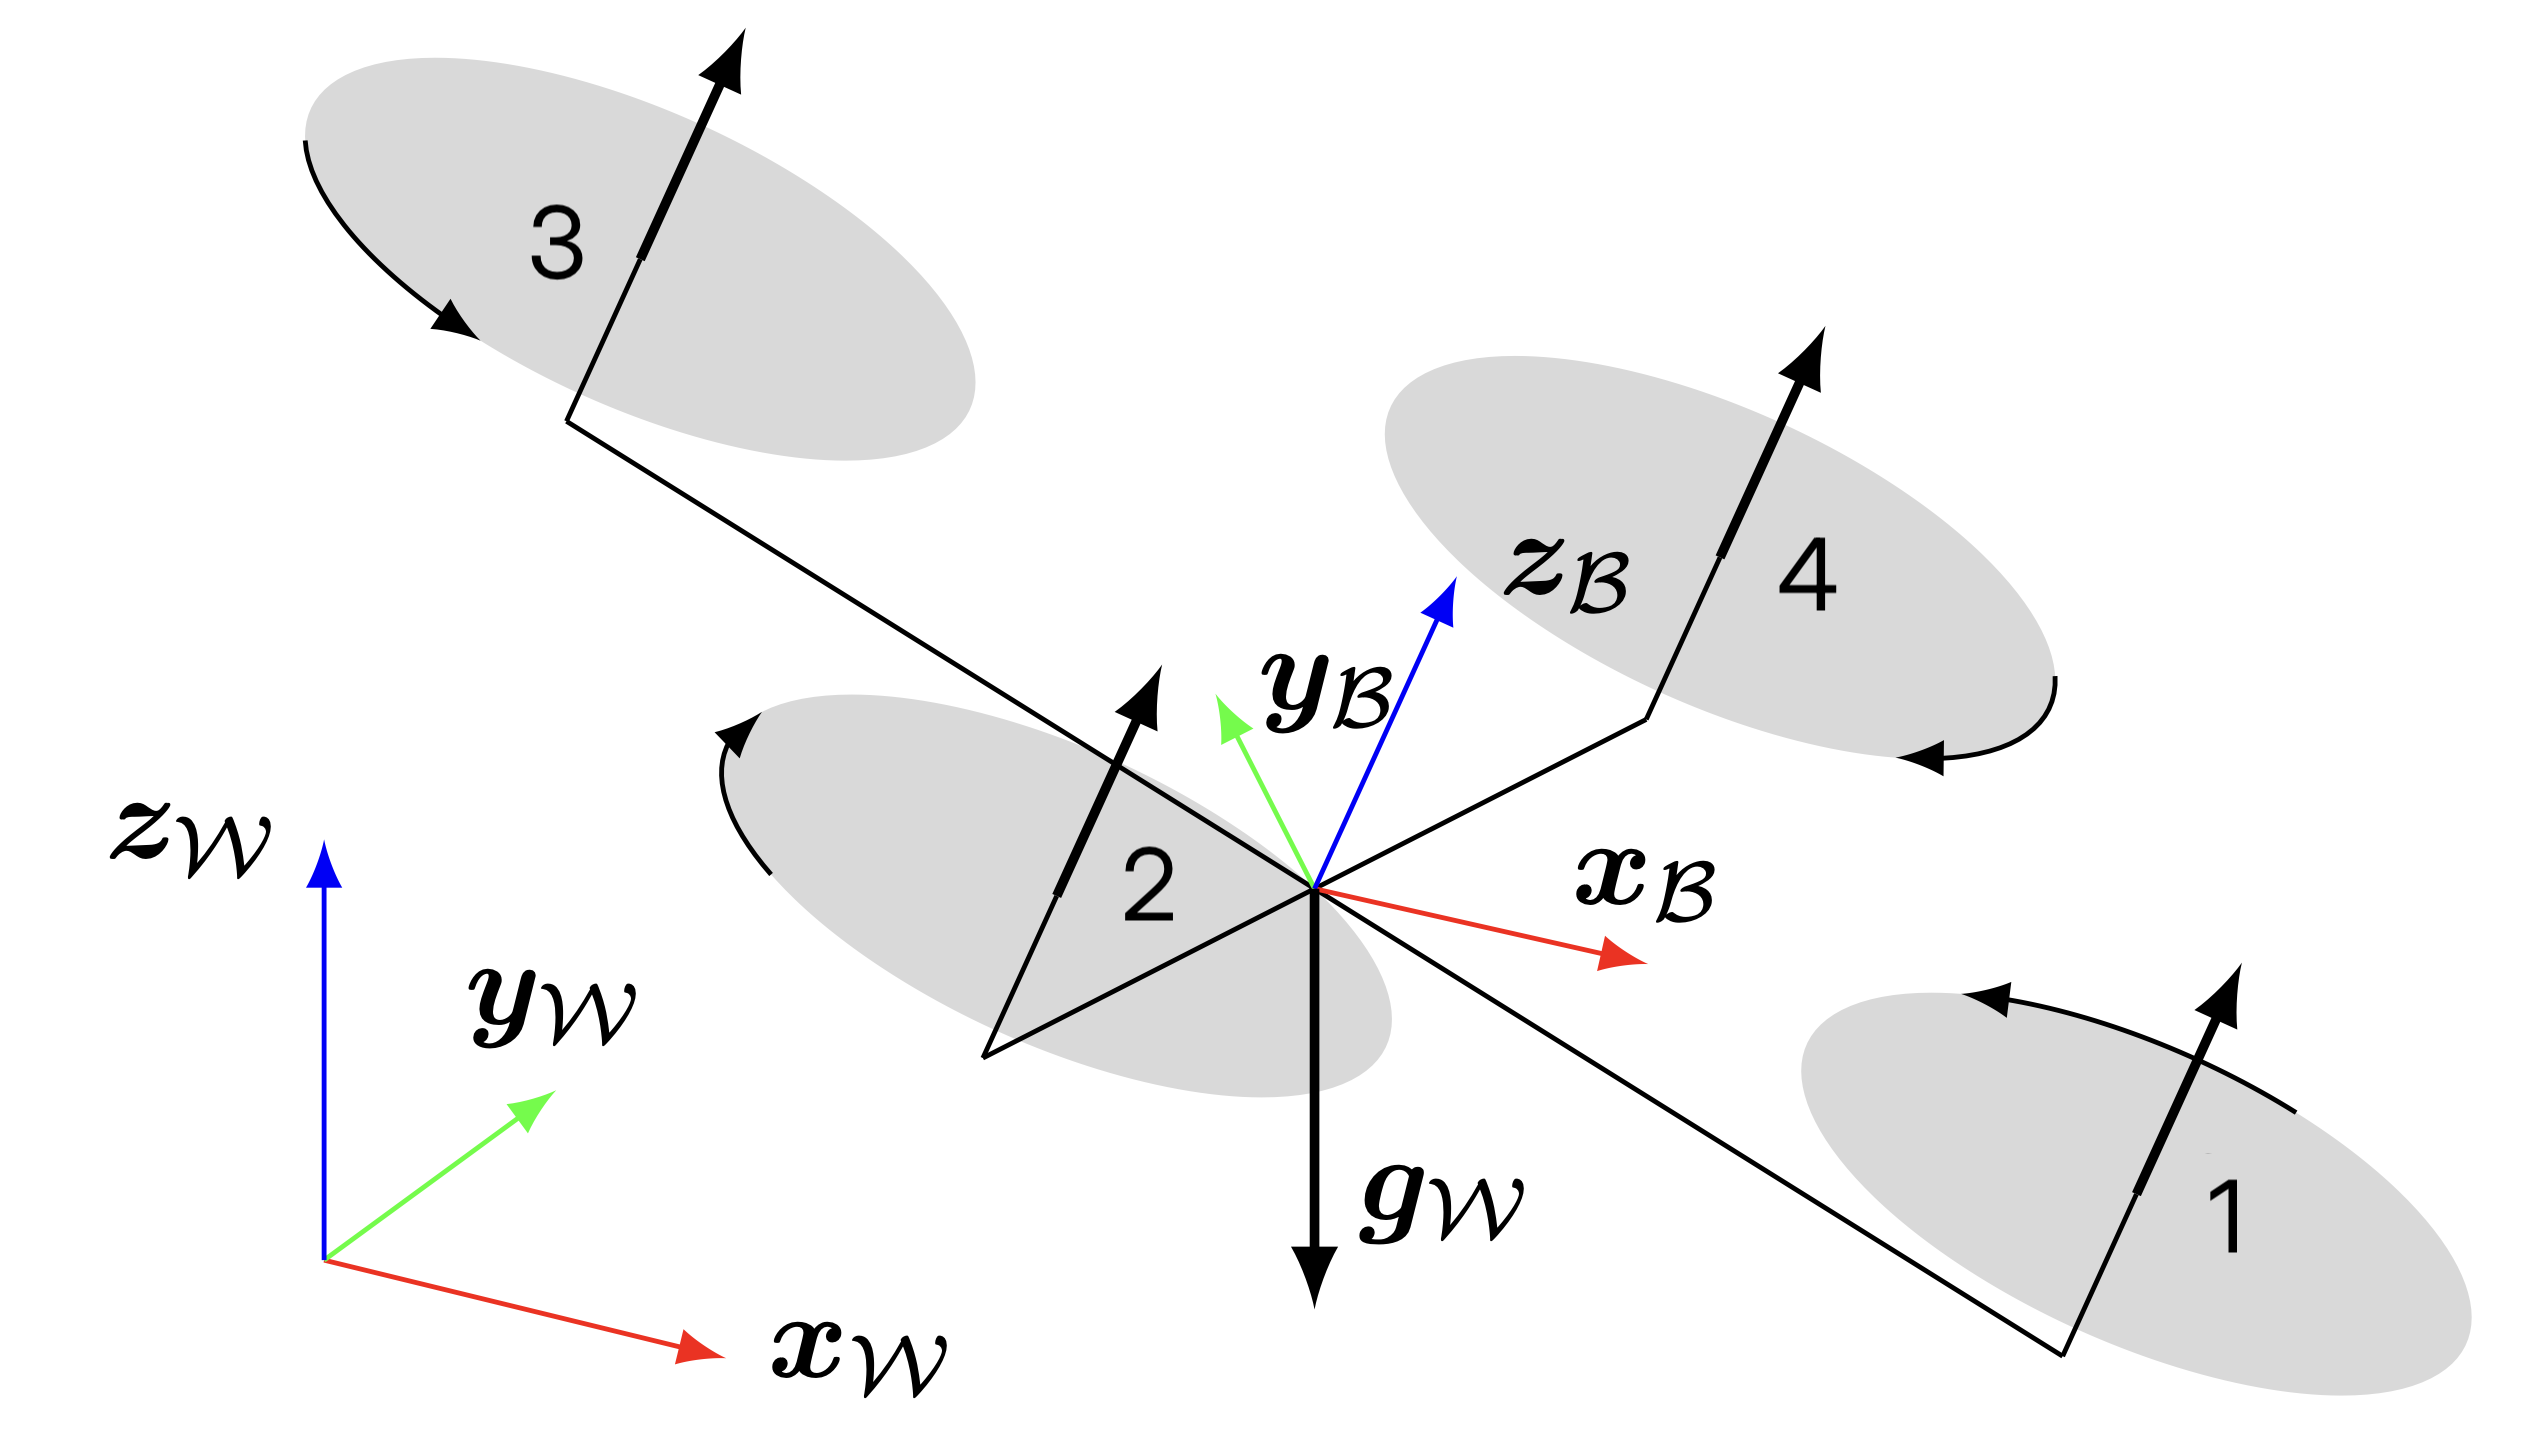
\includegraphics[width=0.5\textwidth]{figs/quad.png}
  \caption[Quadrotor fundamentals]{%
    Quadrotor frames and propeller numbering. The body-fixed frame \(\mathcal{B}\) is centered at the quadrotor's center of mass, with axes aligned to the forward, right, and upward directions. The world frame \(\mathcal{W}\) is a fixed global reference frame. Propellers are numbered 1-4 in a counter-clockwise direction when viewed from above. \textit{Source:} \cite{kaufmann_benchmark_2022}.
  }
  \label{fig:quadrotor_frames}
\end{figure}

\subsection{Coordinate Frames and State Representation}
\label{sec:quadrotor_state}
We define the world frame \(\mathcal{W}\) and the body-fixed frame \(\mathcal{B}\) as shown in Figure~\ref{fig:quadrotor_frames}. The origin of \(\mathcal{B}\) is at the quadrotor's center of mass, with its \(x\)-axis pointing forward, \(y\)-axis to the right, and \(z\)-axis upward. The quadrotor's position in \(\mathcal{W}\) is \(\mathbf{p} \in \mathbb{R}^3\), and its linear velocity is \(\mathbf{v} = \dot{\mathbf{p}}\). Its attitude is given by \(\mathbf{R} \in SO(3)\), mapping vectors from \(\mathcal{B}\) to \(\mathcal{W}\), and the angular velocity in \(\mathcal{B}\) is \(\boldsymbol{\omega} = [\omega_x,\omega_y,\omega_z]^\mathsf{T} \in \mathbb{R}^3\). We collect these into the state
\begin{equation}
x = \bigl(\mathbf{p},\,\mathbf{v},\,\mathbf{R},\,\boldsymbol{\omega}\bigr).
\end{equation}

\subsection{Sensors and State Estimation}
\label{sec:quadrotor_estimation}
The quadrotor's state estimator fuses measurements from a 9-\gls{dof} \gls{imu} and, when available, an external motion capture system. The \gls{imu} provides accelerometer and gyroscope readings:
\begin{equation}
\mathbf{a}_m = \mathbf{R}^\mathsf{T}\bigl(\ddot{\mathbf{p}} - \mathbf{g}\bigr) + \boldsymbol{\nu}_a,\qquad
\boldsymbol{\omega}_m = \boldsymbol{\omega} + \boldsymbol{\nu}_\omega,
\end{equation}
where \(\mathbf{g}=[0,0,9.81]^\mathsf{T}\) and \(\boldsymbol{\nu}_a,\boldsymbol{\nu}_\omega\) are noise terms. In motion-capture environments, position and (optionally) attitude measurements are
\begin{equation}
\mathbf{p}_{\mathrm{mocap}} = \mathbf{p} + \boldsymbol{\nu}_p,\qquad
\mathbf{R}_{\mathrm{mocap}} = \mathbf{R}\bigl(\mathbf{I} + \widehat{\boldsymbol{\nu}_R}\bigr),
\end{equation}
with \(\boldsymbol{\nu}_p,\boldsymbol{\nu}_R\) small errors and \(\widehat{\cdot}\) mapping \(\mathbb{R}^3\) to \(SO(3)\). Stacking these gives the measurement vector
\begin{equation}
\mathbf{y} = \begin{bmatrix}
\mathbf{a}_m^\mathsf{T} & \boldsymbol{\omega}_m^\mathsf{T} & \mathbf{p}_{\mathrm{mocap}}^\mathsf{T} & \mathrm{vec}(\mathbf{R}_{\mathrm{mocap}})^\mathsf{T}
\end{bmatrix}^\mathsf{T} = h(x) + \boldsymbol{\nu}.
\end{equation}
An \gls{ekf} fuses these measurements to produce \(\hat{x} = (\hat{\mathbf{p}},\,\hat{\mathbf{v}},\,\hat{\mathbf{R}},\,\hat{\boldsymbol{\omega}})\) for use by the low-level controllers.
\subsection{Quadrotor Dynamics}
\label{sec:quadrotor_dynamics}
We augment the state \(x=(\mathbf{p},\mathbf{v},\mathbf{R},\boldsymbol{\omega})\) with propeller speeds \(\boldsymbol{\Omega}=[\Omega_1,\Omega_2,\Omega_3,\Omega_4]^\mathsf{T}\), forming
\begin{equation}
x_{\mathrm{full}} = (\mathbf{p},\,\mathbf{v},\,\mathbf{R},\,\boldsymbol{\omega},\,\boldsymbol{\Omega}).
\end{equation}
Let \(m\) be the mass of the quadrotor, and let \(\mathbf{I} = \mathrm{diag}(J_{x},\,J_{y},\,J_{z})\) be its moment-of-inertia matrix expressed in \(\mathcal{B}\). Gravity in \(\mathcal{W}\) is \(g\,\mathbf{e}_{3}\) with \(\mathbf{e}_{3} = [0,\,0,\,1]^{\mathsf{T}}\). Each propeller \(i\) (numbered 1-4 as in Figure~\ref{fig:quadrotor_frames}) produces an upward thrust \(f_{i} \in \mathbb{R}\) along the body-fixed \(z\)-axis and a reactive torque \(\tau_{i}\in \mathbb{R}\) about that same axis. We assume the thrust and drag torque of each propeller scale quadratically with the motor speed:
\begin{equation}
f_{i}(\Omega_{i}) \;=\; c_{\ell}\,\Omega_{i}^{2}, 
\qquad 
\tau_{i}(\Omega_{i}) \;=\; c_{d}\,\Omega_{i}^{2},
\end{equation}
where \(c_{\ell}\) and \(c_{d}\) are the experimentally identified thrust and drag coefficients.

Let \(\mathbf{r}_{P,i}\in \mathbb{R}^{3}\) be the position vector from the body-frame origin to propeller \(i\). We define the total propulsive force in the body frame as
\begin{equation}
\mathbf{f}_{\mathrm{prop}} = \sum_{i=1}^4 f_i\,\mathbf{e}_3^B,
\end{equation}
and the total torque is
\begin{equation}
\boldsymbol{\tau}_{\mathrm{prop}} = \sum_{i=1}^4 \Bigl(\tau_i\,\mathbf{e}_3^B + \mathbf{r}_{P,i}\times(f_i\,\mathbf{e}_3^B)\Bigr).
\end{equation}
Ignoring aerodynamic drag, the continuous-time dynamics are
\begin{equation}
\dot{\mathbf{p}} = \mathbf{v}, 
\qquad
\dot{\mathbf{R}} = \mathbf{R}\,\widehat{\boldsymbol{\omega}},
\end{equation}
\begin{equation}
m\,\dot{\mathbf{v}} = \mathbf{R}\,\mathbf{f}_{\mathrm{prop}} - m\,g\,\mathbf{e}_3,
\end{equation}
\begin{equation}
\mathbf{I}\,\dot{\boldsymbol{\omega}} = \boldsymbol{\tau}_{\mathrm{prop}} - \boldsymbol{\omega} \times (\mathbf{I}\,\boldsymbol{\omega}),
\end{equation}
\begin{equation}
\dot{\boldsymbol{\Omega}} = \tfrac{1}{k_{\mathrm{mot}}}(\boldsymbol{\Omega}_{\mathrm{cmd}} - \boldsymbol{\Omega}),
\end{equation}
where \(\widehat{\boldsymbol{\omega}}\) is the skew-symmetric matrix of \(\boldsymbol{\omega}\), \(k_{\mathrm{mot}}\) is the motor time constant, and \(\boldsymbol{\Omega}_{\mathrm{cmd}}\) is the commanded motor-speed vector \cite{kaufmann_benchmark_2022}.

\subsection{Control Action Parameterizations}
\label{sec:quadrotor_actions}
Following \cite{kaufmann_benchmark_2022}, we describe three common action-space definitions for quadrotor control:

\paragraph{Linear Velocity \& Yaw Rate (LV)}  
An LV policy outputs a desired body-frame velocity \(\mathbf{v}_{\mathrm{des}}=[v_x,v_y,v_z]^\mathsf{T}\) and a yaw rate \(\omega_z\):
\begin{equation}
u_{\mathrm{LV}} = \{v_x,\,v_y,\,v_z,\,\omega_z\}.
\end{equation}
A cascaded low-level controller converts these into collective thrust \(c=\|\mathbf{f}_{\mathrm{prop}}\|\) and attitude setpoints, then allocates individual propeller thrusts \(f_i\) to achieve the commanded \(\omega_z\). LV reduces sample complexity and improves sim-to-real transfer but cannot leverage full force-torque dynamics for aggressive maneuvers.

\paragraph{\glsxtrfull{ctbr}}  
A \gls{ctbr} policy outputs total thrust \(c\in\mathbb{R}\) and body-rate setpoints \(\boldsymbol{\omega}_{\mathrm{des}}=[\omega_x,\omega_y,\omega_z]^\mathsf{T}\):
\begin{equation}
u_{\mathrm{CTBR}} = \{c,\,\omega_x,\,\omega_y,\,\omega_z\}.
\end{equation}
An inner-loop rate controller computes moments \(\mathbf{M}=[M_x,M_y,M_z]^\mathsf{T}\) to track \(\boldsymbol{\omega}_{\mathrm{des}}\), and the mixer solves
\begin{equation}
\sum_{i=1}^4 f_i = c, 
\quad
\ell\,(f_2 - f_4) = M_x, 
\quad
\ell\,(f_3 - f_1) = M_y, 
\quad
\tau_1 - \tau_2 + \tau_3 - \tau_4 = M_z
\end{equation}
for individual thrusts \(f_i\). \gls{ctbr} achieves higher agility than LV while remaining more robust than end-to-end approaches.

\paragraph{\glsxtrfull{srt}}
An \gls{srt} policy outputs the four individual propeller thrusts:
\begin{equation}
u_{\mathrm{SRT}} = \{f_1,\,f_2,\,f_3,\,f_4\},
\end{equation}
where \(f_i = c_\ell \Omega_i^2\). This end-to-end formulation grants full authority over \(\mathbf{f}_{\mathrm{prop}}\) and \(\boldsymbol{\tau}_{\mathrm{prop}}\), enabling the most aggressive maneuvers, but it is sample-inefficient and sensitive to modeling errors.

In summary, LV actions abstract away low-level thrust allocation at the cost of dynamic expressiveness, \gls{ctbr} retains medium-level control over thrust and attitude rates and \gls{srt} provides full end-to-end control at the cost of higher learning complexity and sensitivity to modeling errors.
\section{Quadrotors with Cable-Suspended Payloads}
\label{sec:quadrotor_with_payloads}
\begin{figure}

  \centering
  \begin{subfigure}[t]{0.3\textwidth}
    \centering
    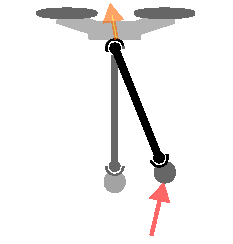
\includegraphics[width=0.8\textwidth]{figs/cable-rod.pdf}
    \caption{Rigid Rod}
  \end{subfigure}
  \begin{subfigure}[t]{0.3\textwidth}
    \centering
    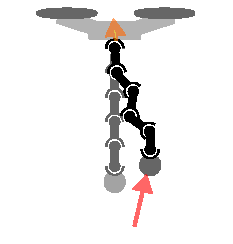
\includegraphics[width=0.8\textwidth]{figs/cable-links.pdf}
    \caption{Multi-link}
  \end{subfigure}
  \begin{subfigure}[t]{0.3\textwidth}
    \centering
    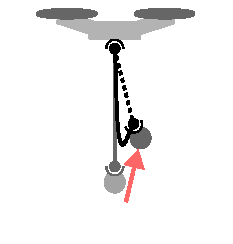
\includegraphics[width=0.8\textwidth]{figs/cable-tendon.pdf}
    \caption{Tendon}
  \end{subfigure}
  \caption[Cable modeling approaches]{Different approaches to modeling a cable-suspended payload. (a) A simple pendulum model with a rigid link and point-mass payload. (b) A multi-link pendulum model with \(N\) serial links. (c) A tendon approximation in MuJoCo. We show how each of these models transfer a upwards disturbance force to the payload (marked in red) to the quadrotor (resulting force in orange). The taut state is shown translucent behind the disturbe state.}
  \label{fig:cable_models}
\end{figure}
We evaluate multiple approaches to modeling quadrotors with cable-suspended payloads, which are common in aerial manipulation and transport tasks. These models extend the quadrotor state to include cable and payload variables, enabling simulation and control of cooperative transport scenarios. Figure~\ref{fig:cable_models} illustrates three common modeling approaches: a simple rigid-rod pendulum, a multi-link pendulum, and a tendon approximation in MuJoCo.

A simple rigid-rod pendulum model treats the cable as a massless, inextensible rigid link of length \(\ell\) with a point-mass payload \(m_L\). The payload position \(\mathbf{p}_L\) relates to the quadrotor position \(\mathbf{p}_Q\) via
\begin{equation}
\mathbf{p}_L = \mathbf{p}_Q - \ell\,\mathbf{q}, 
\quad
\|\mathbf{q}\| = 1,
\end{equation}
where \(\mathbf{q}\in S^2\) is the unit vector along the cable \cite{estevez_review_2024}. The augmented state is
\begin{equation}
x_{\mathrm{aug}} = (\mathbf{p}_Q,\,\mathbf{v}_Q,\,\mathbf{R},\,\boldsymbol{\omega},\,\mathbf{q},\,\dot{\mathbf{q}}),
\end{equation}
with \(\mathbf{v}_Q = \dot{\mathbf{p}}_Q\) and \(\dot{\mathbf{q}}\) capturing payload swing \cite{Wahba2024}.

A multi-link pendulum model represents the cable as \(N\) serial, massless links of lengths \(\{\ell_i\}\), each with orientation \(\mathbf{q}_i\in S^2\). The payload position becomes
\begin{equation}
\mathbf{p}_L = \mathbf{p}_Q - \sum_{i=1}^N \ell_i\,\mathbf{q}_i,
\end{equation}
and the state is augmented by \(\{\mathbf{q}_i,\,\dot{\mathbf{q}}_i\}_{i=1}^N\). This captures cable sag and higher-order swing modes but increases the state dimension from 8 (rigid link) to \(6+4N\), where 6 corresponds to \(\mathbf{p}_Q,\,\mathbf{v}_Q,\,\mathbf{R},\,\boldsymbol{\omega}\) \cite{goodarzi_dynamics_2015}.

In MuJoCo, cables are approximated as tendon elements—massless, inelastic, high-stiffness springs enforcing \(\|\mathbf{p}_Q - \mathbf{p}_L\| = \ell\) when taut and acting as slack otherwise. The augmented state is
\begin{equation}
x_{\mathrm{aug}} = (\mathbf{p}_Q,\,\mathbf{v}_Q,\,\mathbf{R},\,\boldsymbol{\omega},\,\mathbf{p}_L,\,\mathbf{v}_L),
\end{equation}
where \(\mathbf{v}_L = \dot{\mathbf{p}}_L\). Tendon tension \(\mathbf{T}\) applies \(-\mathbf{T}\) on the quadrotor and \(+\mathbf{T}\) on the payload.

For cooperative transport with \(M\) quadrotors, each quadrotor \(i\) connects to a common payload of mass \(m_P\) via its own tendon. The payload dynamics are
\begin{equation}
m_P \,\ddot{\mathbf{p}}_P = -m_P\,\mathbf{g} + \sum_{i=1}^M \mathbf{T}_i,
\end{equation}
and each quadrotor's translational dynamics include \(-\mathbf{T}_i\) alongside its thrust. The joint state is
\begin{equation}
x_{\mathrm{aug}} = \bigl(\{\mathbf{p}_i,\,\mathbf{v}_i,\,\mathbf{R}_i,\,\boldsymbol{\omega}_i\}_{i=1}^M,\,\mathbf{p}_P,\,\mathbf{v}_P\bigr),
\end{equation}
capturing multi-agent interactions, payload swing, tension variations, and hybrid dynamics while remaining computationally efficient for simulation and control experiments.

For our work we model the cable as a tendon. The key distinction of the tendon model is that it only applies forces when the cable is taut and in tension, while the rigid rod and multi-link models forward forces even when the cable is slack as illustrated in Figure~\ref{fig:cable_models}. This difference is particularly significant in the interaction of the system with the ground and in the interplay between the quadrotors in a very dynamic movement.